\subsection{概要}
三重県内のある地域では,処方薬の重複や過剰投与を避けるために
投薬に関する情報を共有したいという要望があがっている.
これを受け,投薬データとその根拠になっていると考えられる
検査データを共有することができるシステムを開発する.
データ入力は鈴鹿医療科学大学から提供していただいた検査データと投薬データ
のみを受け付ける.よってデータベースにはSQLデータベースを用いて
投薬データを書き込むテーブルと,検査データを書き込むテーブルを用意する.

\subsection{機能}
  \subsubsection{権限の付与}
    図\ref{DjangoFileio}は患者がシステムにログインした後の画面である.
    図の中段の「relationを追加する」フォームで医療関係者のIDを
    入力することで,
    患者の医療情報をどの医療関係者が操作することができるかを
    患者自身が選択する.


  \subsubsection{データ入力}
    データベースには提供していただいたエクセルファイルの記述方法に対応する
    SQLのテーブルを用意している.
    ファイルをアプリケーションが図\ref{DjangoFileio}の
    ページで受け取ると検査値と投薬についての
    情報を医療情報をデータベースへ入力することができる.

  \subsubsection{データ閲覧}
    診断データは表にして、縦方向に診断項目,
    横方向に診断を行った日をとっている.
    空白部分はデータが入力されていない項目である.
    (図\ref{DjangoTable})


    投薬データはある薬をどれだけの期間服用しているかを
    わかりやすくするためにガントチャートのように表示している.
    色によってカテゴリの視認性を向上させたため,
    複数の医療機関にかかっている際に発生する可能性がある
    同時に服用することが好ましくない薬の組み合わせや
    過度な投薬を医療関係者が発見しやすい.(図\ref{DjangoGantt})



    \begin{figure}[htbp]
      \begin{center}
        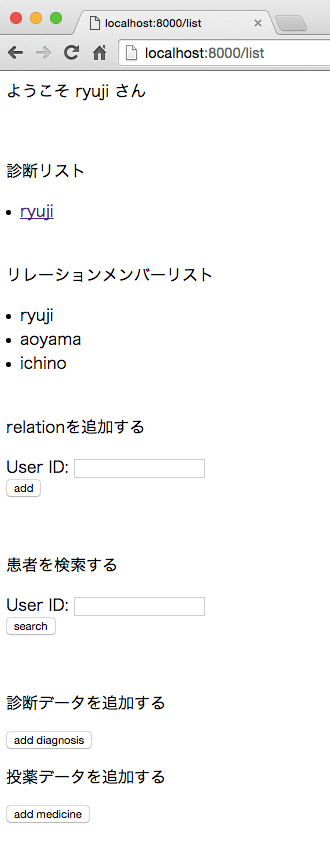
\includegraphics[width=7cm, bb=0 0 330 851, clip]{./gazou/DjangoFileio2.png}
      \end{center}
      \caption{データ入力画面}
      \label{DjangoFileio}
    \end{figure}

    \begin{figure}[htbp]
        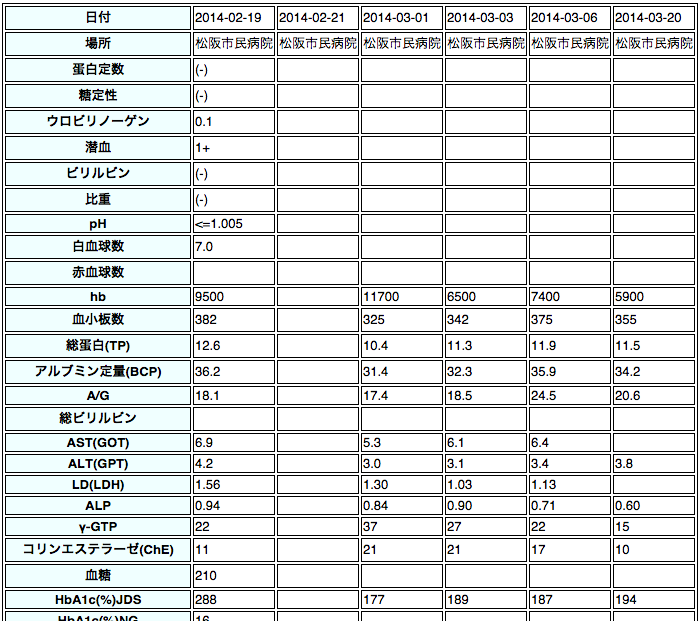
\includegraphics[width=15cm, bb=0 0 698 621]{./gazou/DjangoTable2.png}
      \caption{表によるデータ閲覧}
      \label{DjangoTable}
    \end{figure}

    \begin{figure}[htbp]
        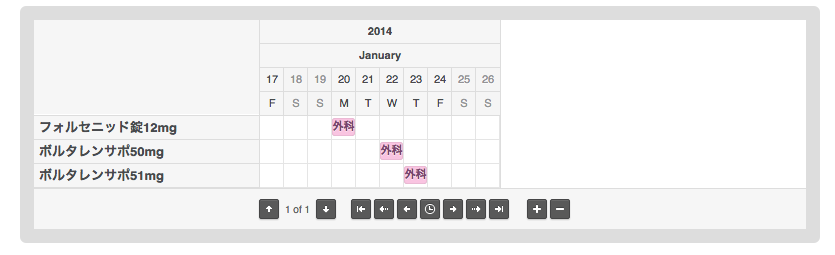
\includegraphics[width=15cm, bb=0 0 835 221]{./gazou/DjangoGantt2.png}
      \caption{ガントチャートによるデータ閲覧}
      \label{DjangoGantt}
    \end{figure}



\subsection{まとめ}
  認可を出す機能に関しては,患者に合わせて柔軟に対応する必要があると考えられる.
  閲覧不可,閲覧可能と書き込み可能の3段階の認可を用意することで
  患者が望む自身の情報の共有のされ方を実現することである.
  これにより,医療関係者は患者の意志を尊重しながら
  医療情報を活用して処方や診断を行うことができる.

  医療情報の入出力に関しては,特定の形式の入力データを受け付けて
  医療情報をグラフィカルに表示することができた.
  これにより投薬の必要性を見直したり,
  重複を避けることができると考えられる.
  また,患者が自身の投薬情報を確認できるので
  どの薬をどれだけの量をいつまで飲まなければならないか
  確認することもできる.
